\chapter{Felhasználói dokumentáció}
\label{ch:user}

A következő fejezetben fogom bemutatni az alkalmazás elérését, egyes komponenseit, illetve felhasználási lehetőségeit. 

Ez a pénzügyeket rendszerező alkalmazás alapvetően magánszemélyeknek készült, személyes felhasználásra, de mivel lehetőséget nyújt csoportos használatra is, ezáltal akár egy kisebb vállalat igényeit is elláthatja.

A főbb funkciók közé tartozik, hogy bevételeket és kiadásokat lehet rögzíteni, kategóriák szerint csoportosítva, illetve kimutatásokat nézhet a felhasználó a pénzügyi szokásairól, melyeket exportálni is tudja. Az alkalmazás egyik nagy előnye, hogy nem csak egyének használhatják, hanem csoportok (például háztartások) is.


\section{Rendszerkövetelmények}

Mivel egy webes alkalmazásról van szó, ezért különleges gépigény nem szükséges. Szinte az összes böngésző támogatott, ahogyan azt a \ref{tab:browsers}. táblázat is mutatja.\footnote{Megjegyzés: Mivel a Microsoftnak nem található hivatalos adata a böngészők legrégebbi támogatott verzióira, ezért a táblázat csupán egy általános modern web applikáció böngésző kritériumait mutatja.}
\begin{table}[H]
	\centering
	\begin{tabular}{ | m{0.25\textwidth} | m{0.25\textwidth} | m{0.35\textwidth} | }
		\hline
		\textbf{Böngésző} & \textbf{Minimum Verzió} & \textbf{Támogatás} \\
		\hline
		Google Chrome & 70+ & Teljes \\
		\hline
		Mozilla Firefox & 68+ & Teljes \\
		\hline
		Microsoft Edge (Chromium) & 79+ & Teljes (a régi Edge (EdgeHTML) nem támogatott) \\
		\hline
		Safari & 13+ & Teljes \\
		\hline
		Opera & 57+ & Teljes \\
		\hline
		Internet Explorer & Nem alkalmazható & Nem támogatott a .NET 8-ban \\
		\hline
	\end{tabular}
	\caption{Böngésző Támogatás}
	\label{tab:browsers}
\end{table}

\section{Felhasználói esetek}
Az alkalmazás felhasználói eseteit ez a bejegyzés fogja taglalni jobban, képernyőképekkel magyarázva.

\subsection{Fiók}
A felhasználói fiókok kezelése egy klasszikus Regisztráció-Bejelentkezés-Profil hármasban került kialakításra. A felhasználónak a webalkalmazás elérése érdekében regisztrálnia kell , majd sikeres regisztrációt követően bejelentkezhet a felületre (részletes kifejtés: <<>>). A belső oldalra érve elérhető egy "Profil" oldal a bal menüsávból is, illetve a jobb felső sarokban az ember ikonra kattintva a legördülő menüből is kiválaszható ez a menüpont. Szintén ezen a két helyen találjuk a kijelentkezés gombot is, amellyel megszüntethetjük az adott munkamenetet és kiléphetünk a fiókból. Ezen funkciók részletes leírását a \ref{tab:account}. táblázat foglalja össze.
\begin{table}[H]
	\centering
	\begin{tabular}{ | m{0.25\textwidth} | m{0.65\textwidth} | }
		\hline
		\textbf{Funkció} & \textbf{Leírás} \\
		\hline \hline
		\emph{Bejelentkezés} & Bejelentkezés egy egyedi felhasználónévvel és egy jelszóval lehetséges. (\ref{fig:login}. ábra) \\
		\hline
		\emph{Regisztráció} &  Regisztrálni lehet az oldalra a következő adatok megadásával: e-mail cím, felhasználónév (egyedi), teljes név, jelszó. (\ref{fig:register}. ábra)  \\
		\hline
		\emph{Profil} & A Profil oldalon lehet a fiókhoz tartozó adatokat módosítani: a felhasználónevet, a teljes nevet, illetve az e-mail címet is. Itt elérhető még egy "Change Pass" gomb is, amely elnavigálja a felhasználót a jelszó megváltoztató felületre. A profil oldal használatát a \ref{tab:profile}. táblázat fejti ki bővebben. (\ref{fig:profile}. ábra) \\
		\hline
		\emph{Jelszó módosítás} & A Profil oldalról lehet a jelszó változtató felületet elérni a "Change Pass" gomb megnyomásával. Itt meg kell adni a következő adatokat: régi jelszó, új jelszó, új jelszó megerősítése. \\
		\hline
		\emph{Kijelentkezés} & Ha a felhasználó befejezte kívánt tevékenységét, akkor a bal oldali menüsáv alján található "Logout" gomb megnyomásával tud kijelentkezni. A kijelentkező gomb még elérhető a jobb felső sarokban található ember ikonra kattintva legördülő menüben is. \\
		\hline
	\end{tabular}
	\caption{Fiók műveletek}
	\label{tab:account}
\end{table}

\begin{figure}[H]
	\centering
	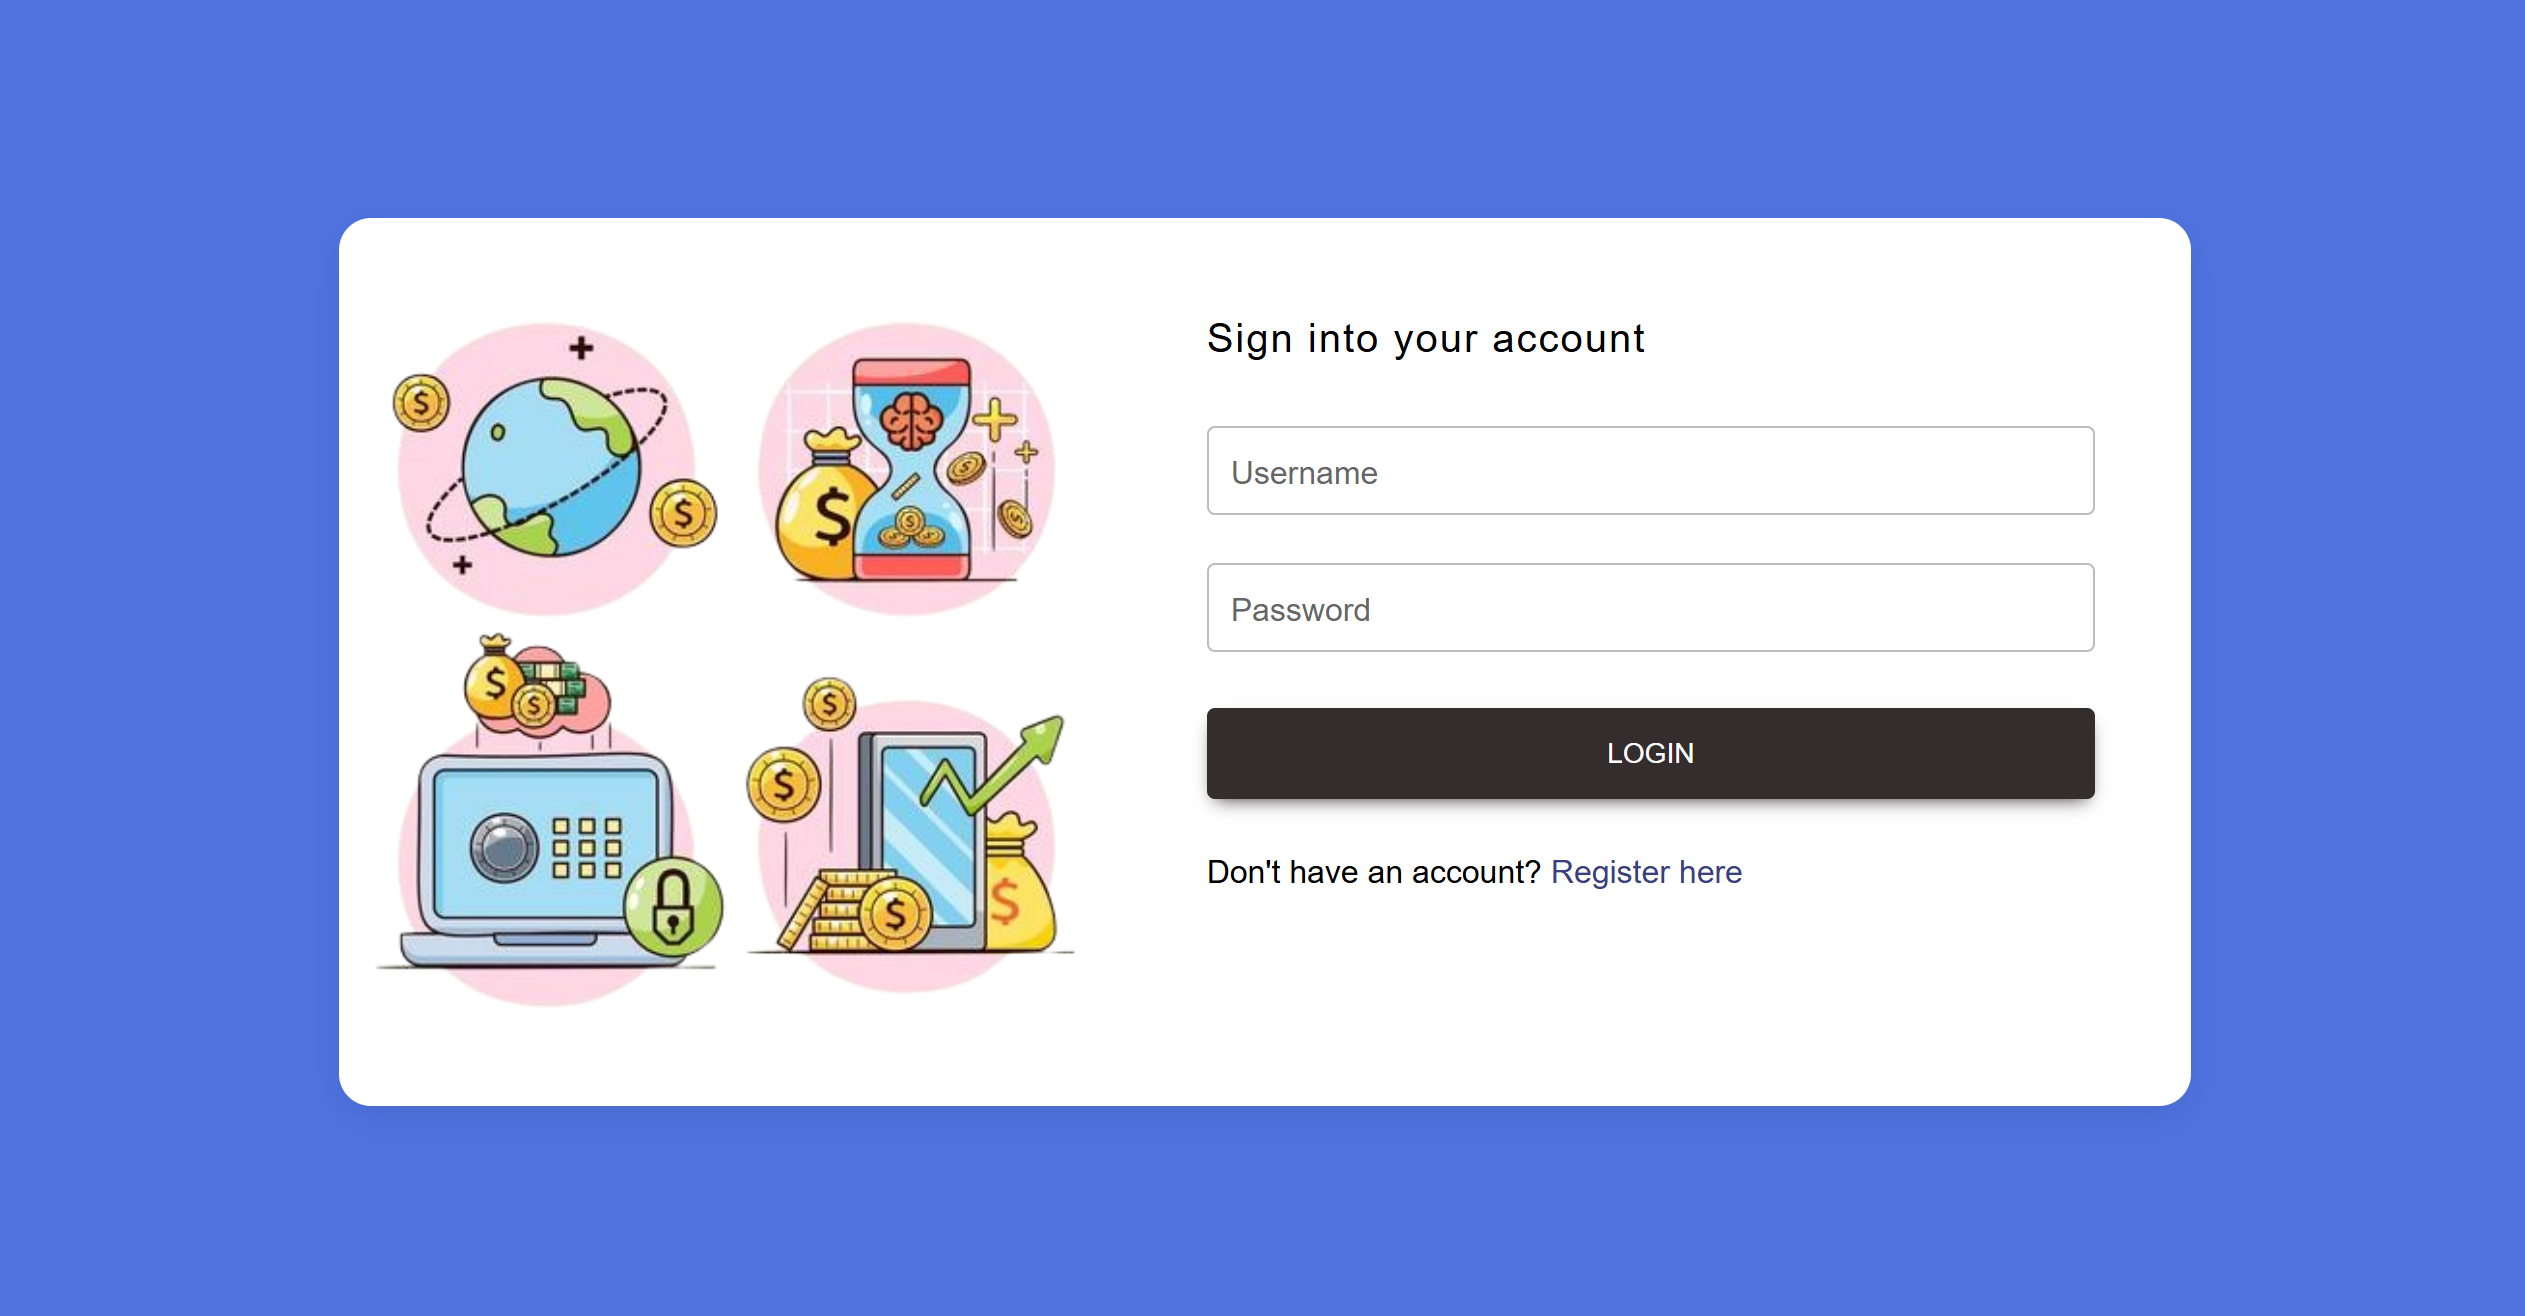
\includegraphics[height=180px]{img/login}
	\caption{Screenshot: Bejelentkező felület}
	\label{fig:login}
\end{figure}

\begin{figure}[H]
	\centering
	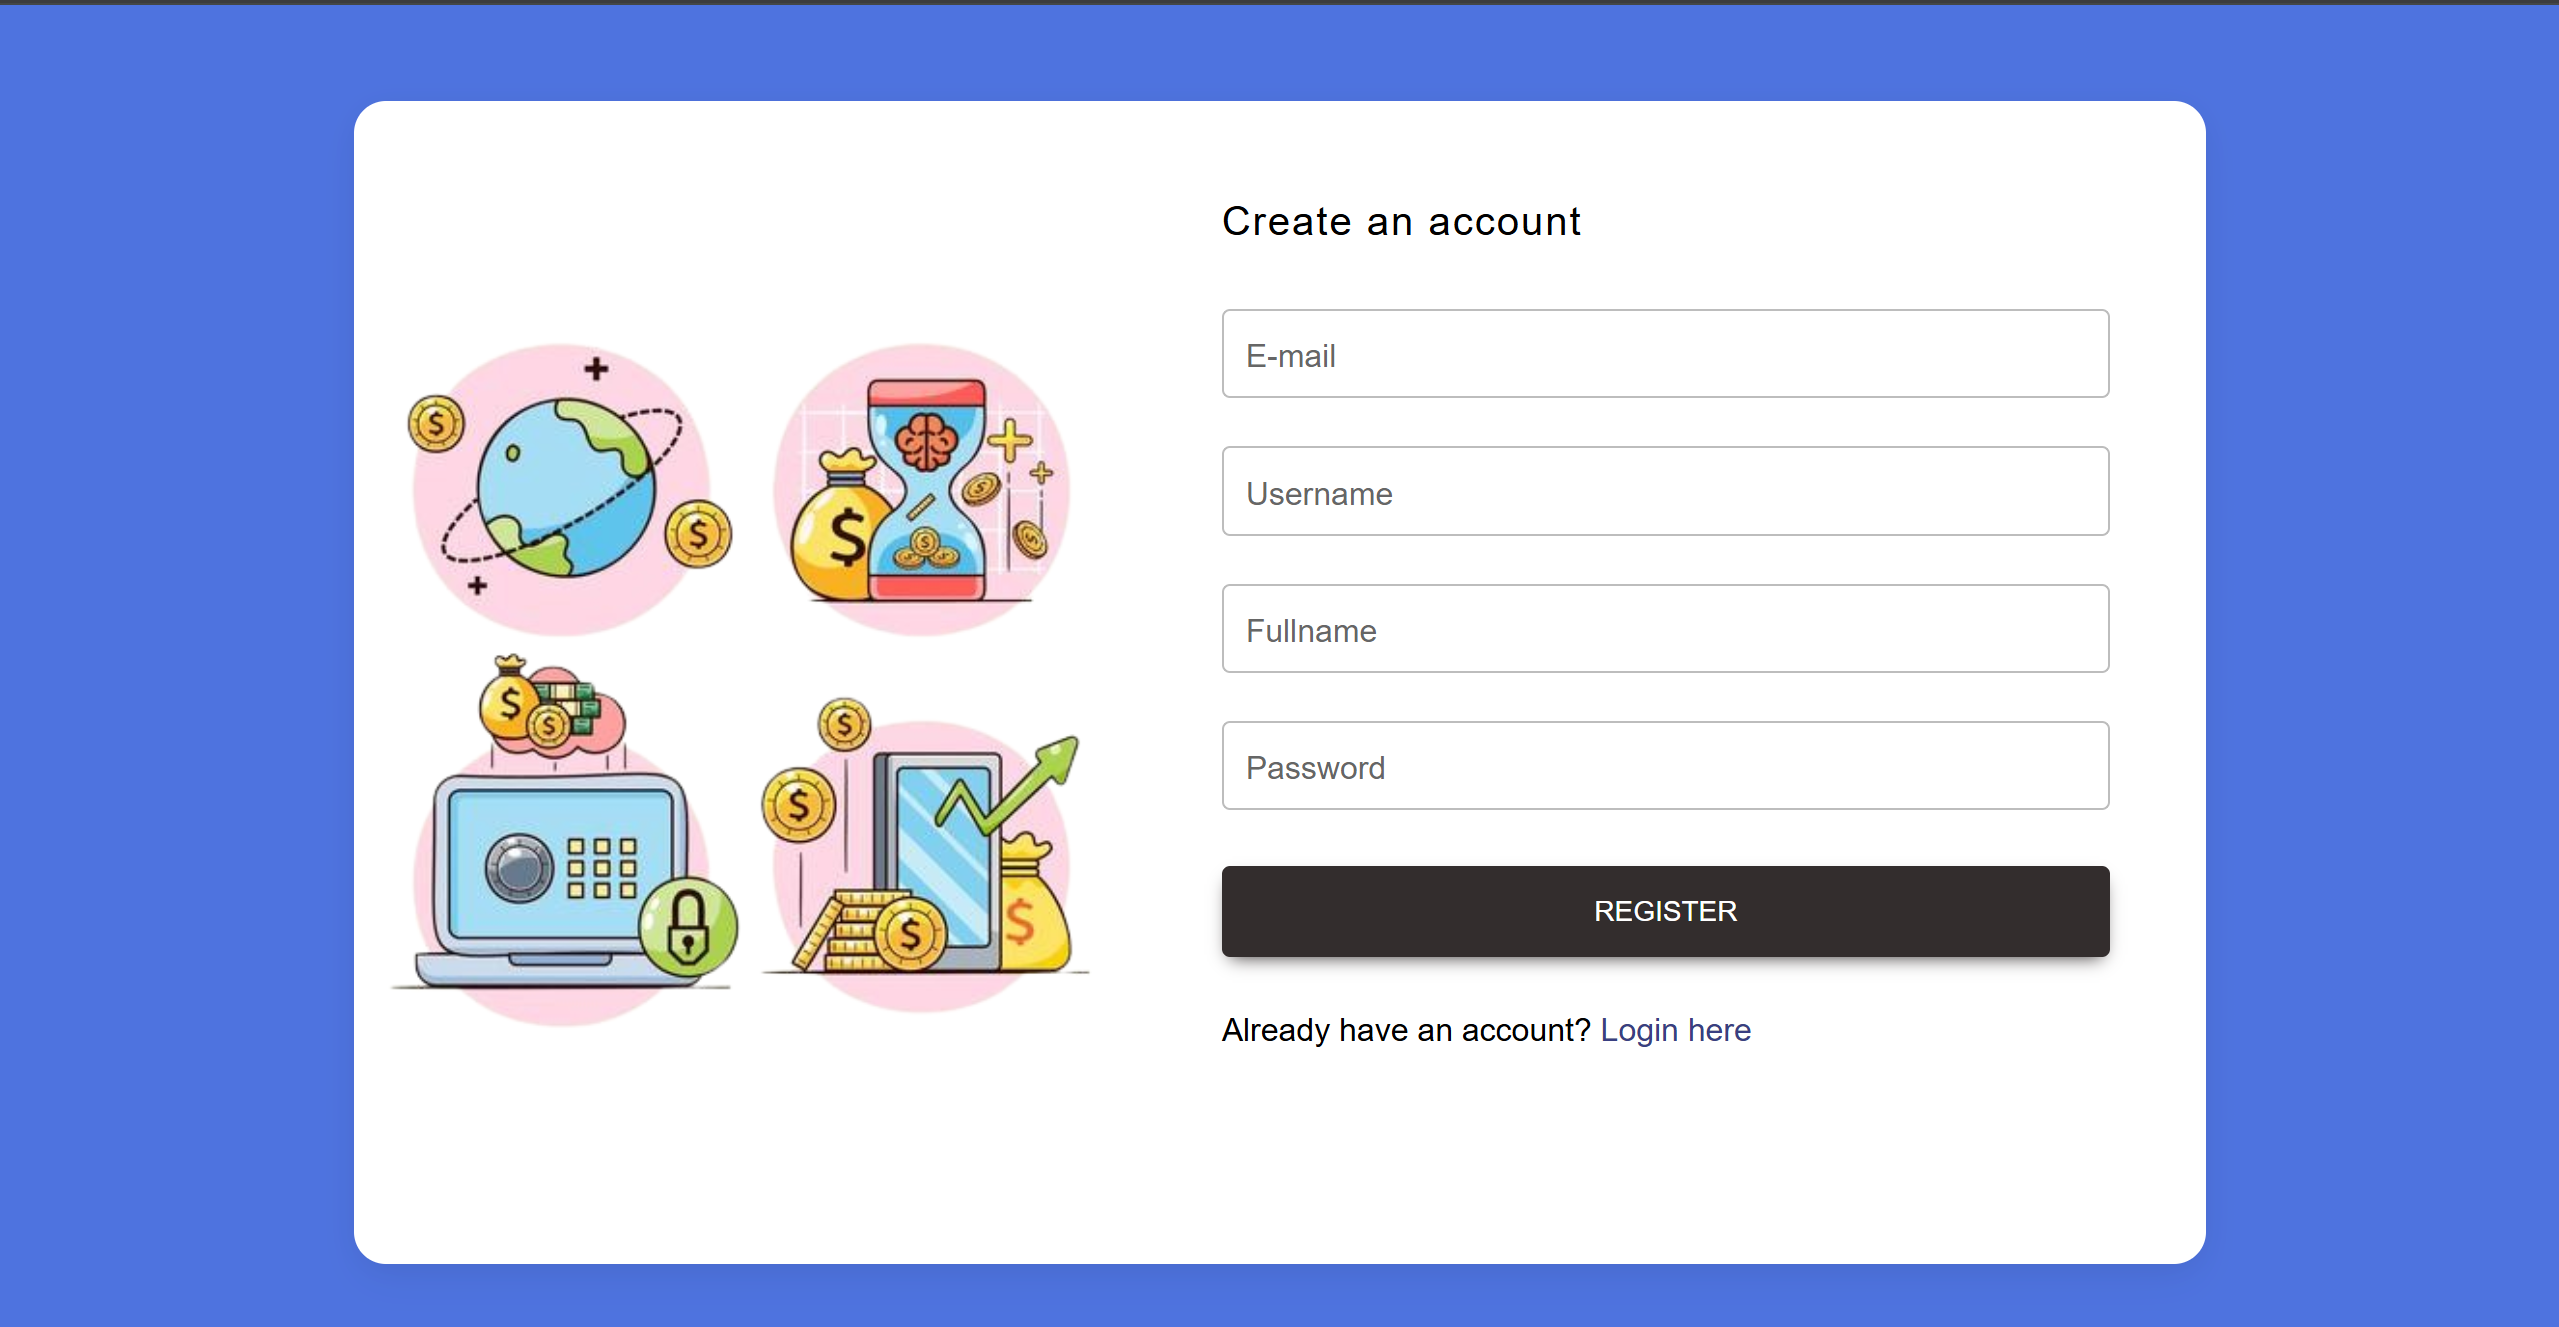
\includegraphics[height=180px]{img/register}
	\caption{Screenshot: Regisztrációs felület}
	\label{fig:register}
\end{figure}

\subsection{Profil}
A profil oldalt a bal menüsávből érhetjük el.
\begin{table}[H]
	\centering
	\begin{tabular}{ | m{0.25\textwidth} | m{0.65\textwidth} | }
		\hline
		\textbf{Funkció} & \textbf{Leírás} \\
		\hline \hline
		\emph{Adatok megtekintése} & A regisztrációnál megadott személyes adatait a felhasználó itt tekintheti meg. \\
		\hline
		\emph{Adatok módosítása} &  A személyes adatok módosítására is itt van lehetőség, egyszerű beviteli mezőkkel lehet módosítani a felhasználónevet (egyedi), teljes nevet és e-mail címet. A "Change" gombra kattintva előugrik egy beviteli mező egy "Save" és "Cancel" gombbal kiegészítve. Az előbbi megpróbálja végrehajtani a kért módosítást, és jelzi az esetlegesen fellépő hibát (érvénytelen e-mail cím, foglalt felhasználónév, stb.) a felhasználó felé.  \\
		\hline
		\emph{Jelszó módosítás} & Ha a felhasználó módosítani kívánja a jelszavát, akkor a "Change Password" gombra kattintva megjelenik egy új felület, három szerveren is validált jelszó beviteli mezővel (régi, új, új megerősítése). \\
		\hline
	\end{tabular}
	\caption{Profil oldal}
	\label{tab:profile}
\end{table}

\begin{figure}[H]
	\centering
	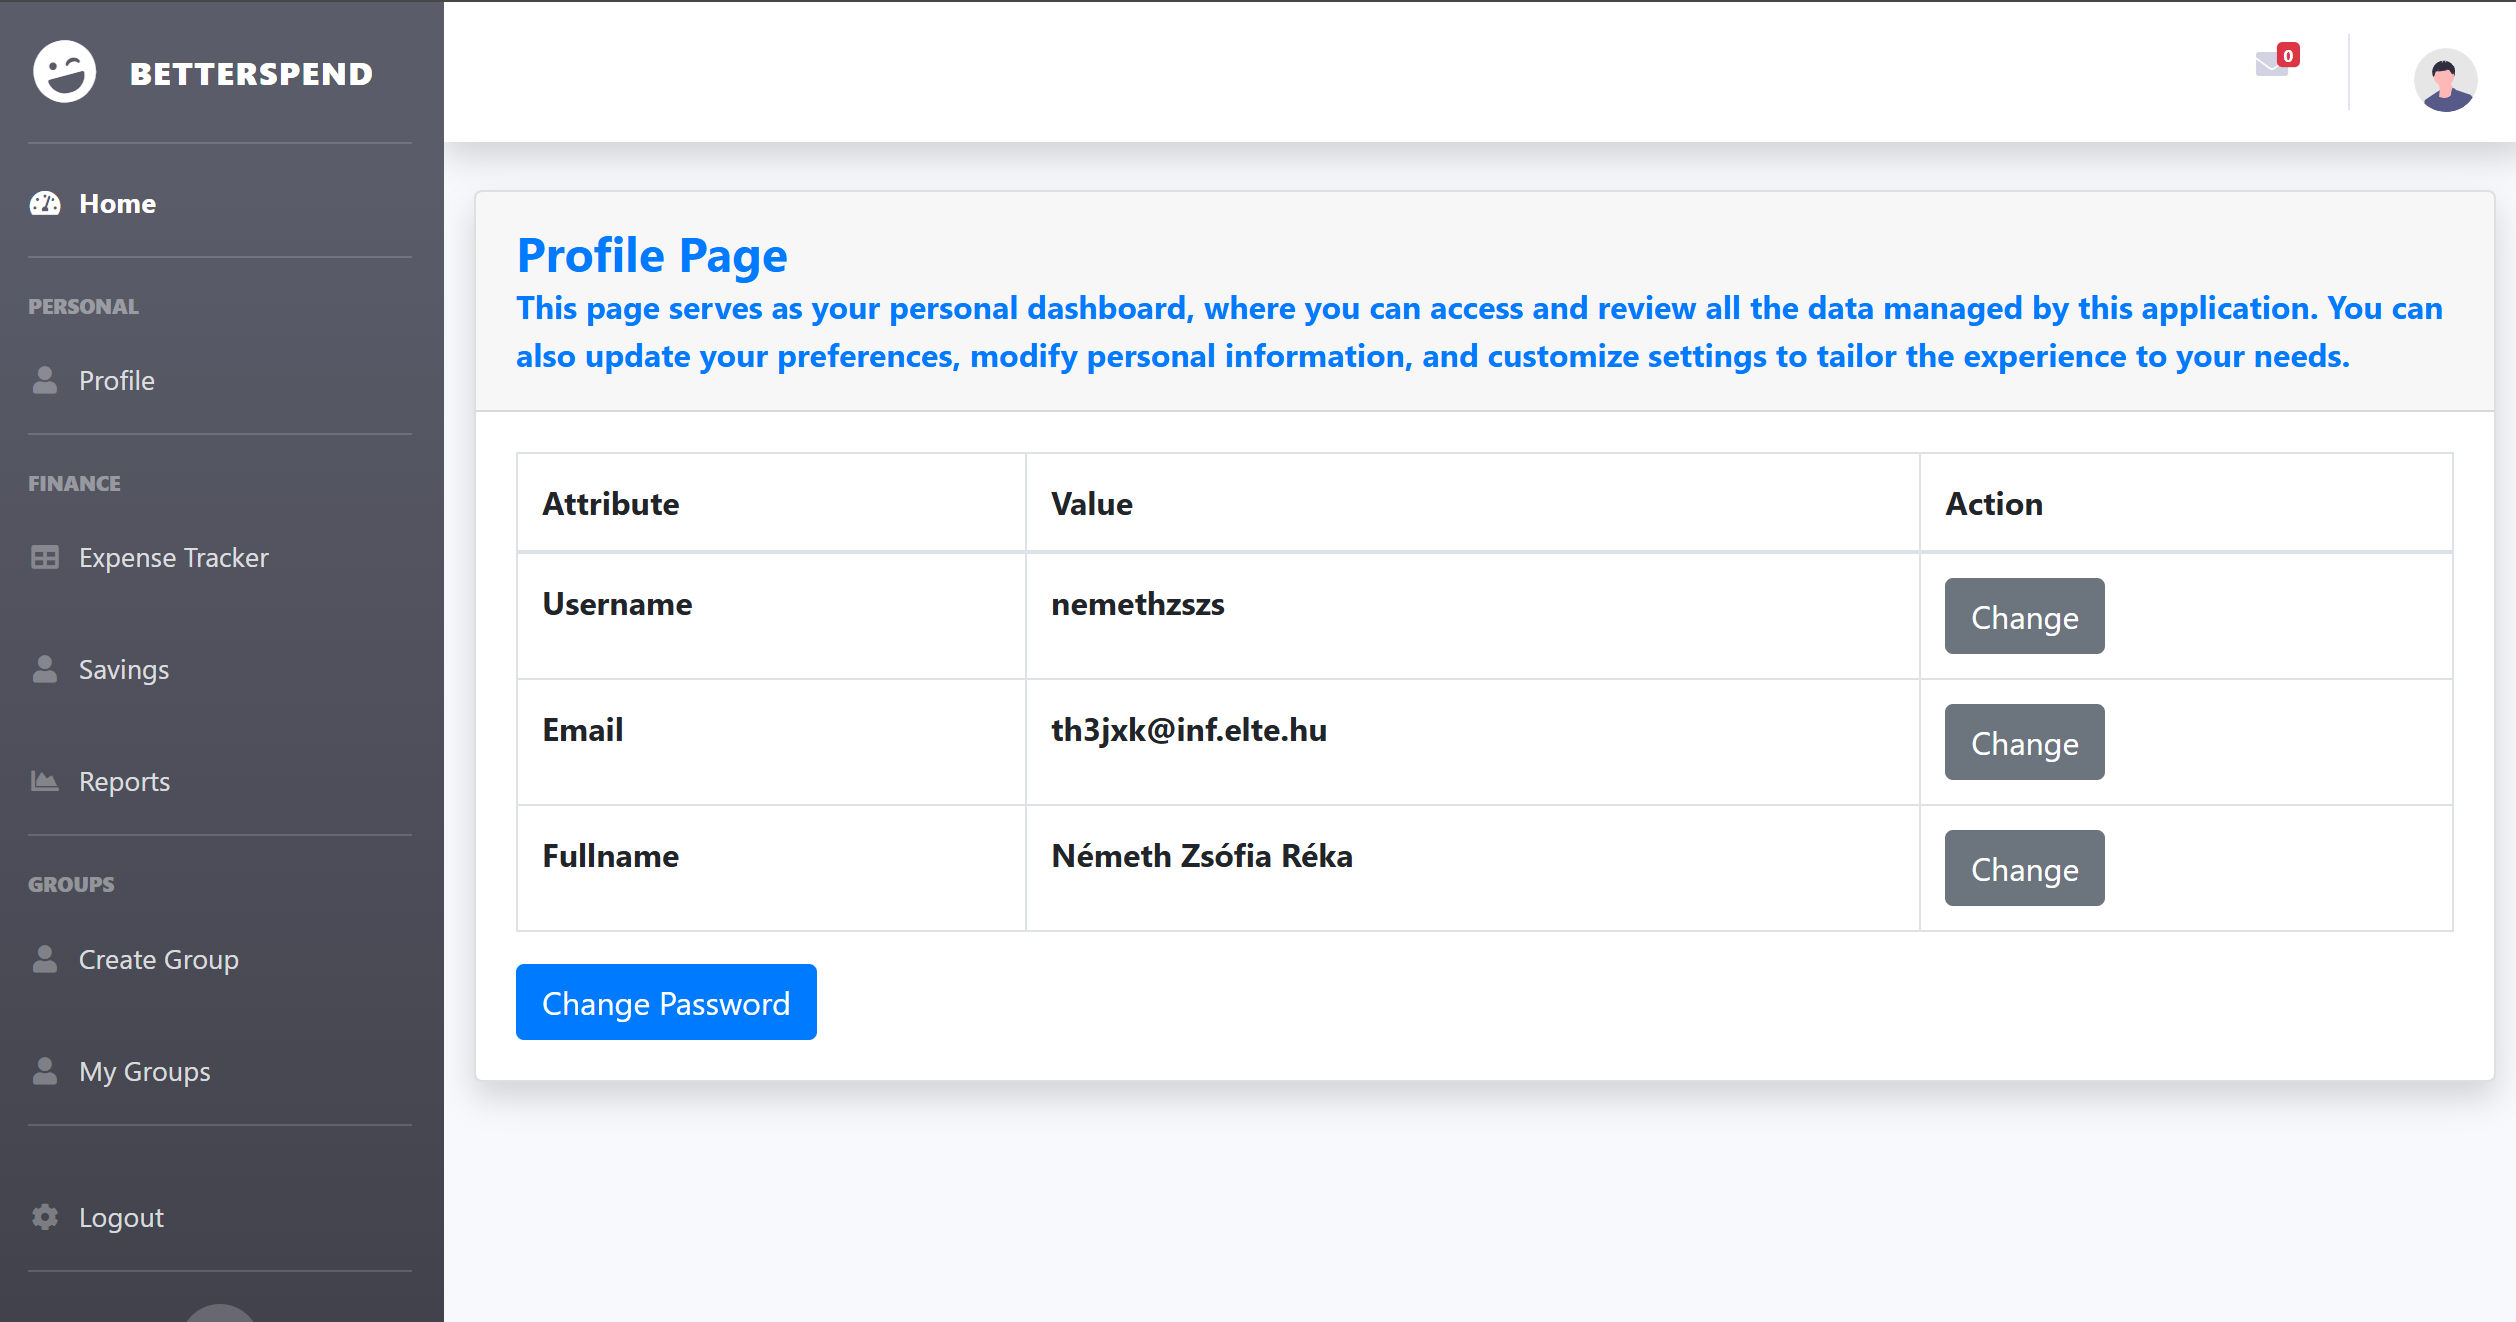
\includegraphics[height=190px]{img/profile}
	\caption{Screenshot: Profil felület}
	\label{fig:profile}
\end{figure}

\subsection{Pénzügyek}
A pénzügyeket kezelő oldalakat a bal menüsávből érhetjük el. Ezen a főmenüponton belül is 3 almenüpont lett kialakítva: 
\begin{itemize}
	\item Expense Tracker (Bevételek és kiadások vezetése, és előzmények megtekintése)
	\item Savings (Megtakarítások megtekintése és kezelése)
	\item Reports (Kimutatások megtekintése, személyre szabása és exportálása)
\end{itemize}

\begin{table}[H]
	\centering
	\begin{tabular}{ | m{0.25\textwidth} | m{0.65\textwidth} | }
		\hline
		\textbf{Funkció} & \textbf{Leírás} \\
		\hline \hline
		\emph{Kiadás/bevétel rögzítése} & Külön dobozokban lehet rögzíteni a kiadásokat, és a bevételeket. Egyszerre egyet lehet bevinni, melynek adni kell egy összeget, egy leírást, opcionálisan lehet kategóriát is megadni. \\
		\hline
		\emph{Előzmények} &  A költési és bevételi előzményeket is itt lehet megtekinteni.  \\
		\hline
	\end{tabular}
	\caption{Expense Tracker oldal}
	\label{tab:expense-tracker}
\end{table}

\begin{figure}[H]
	\centering
	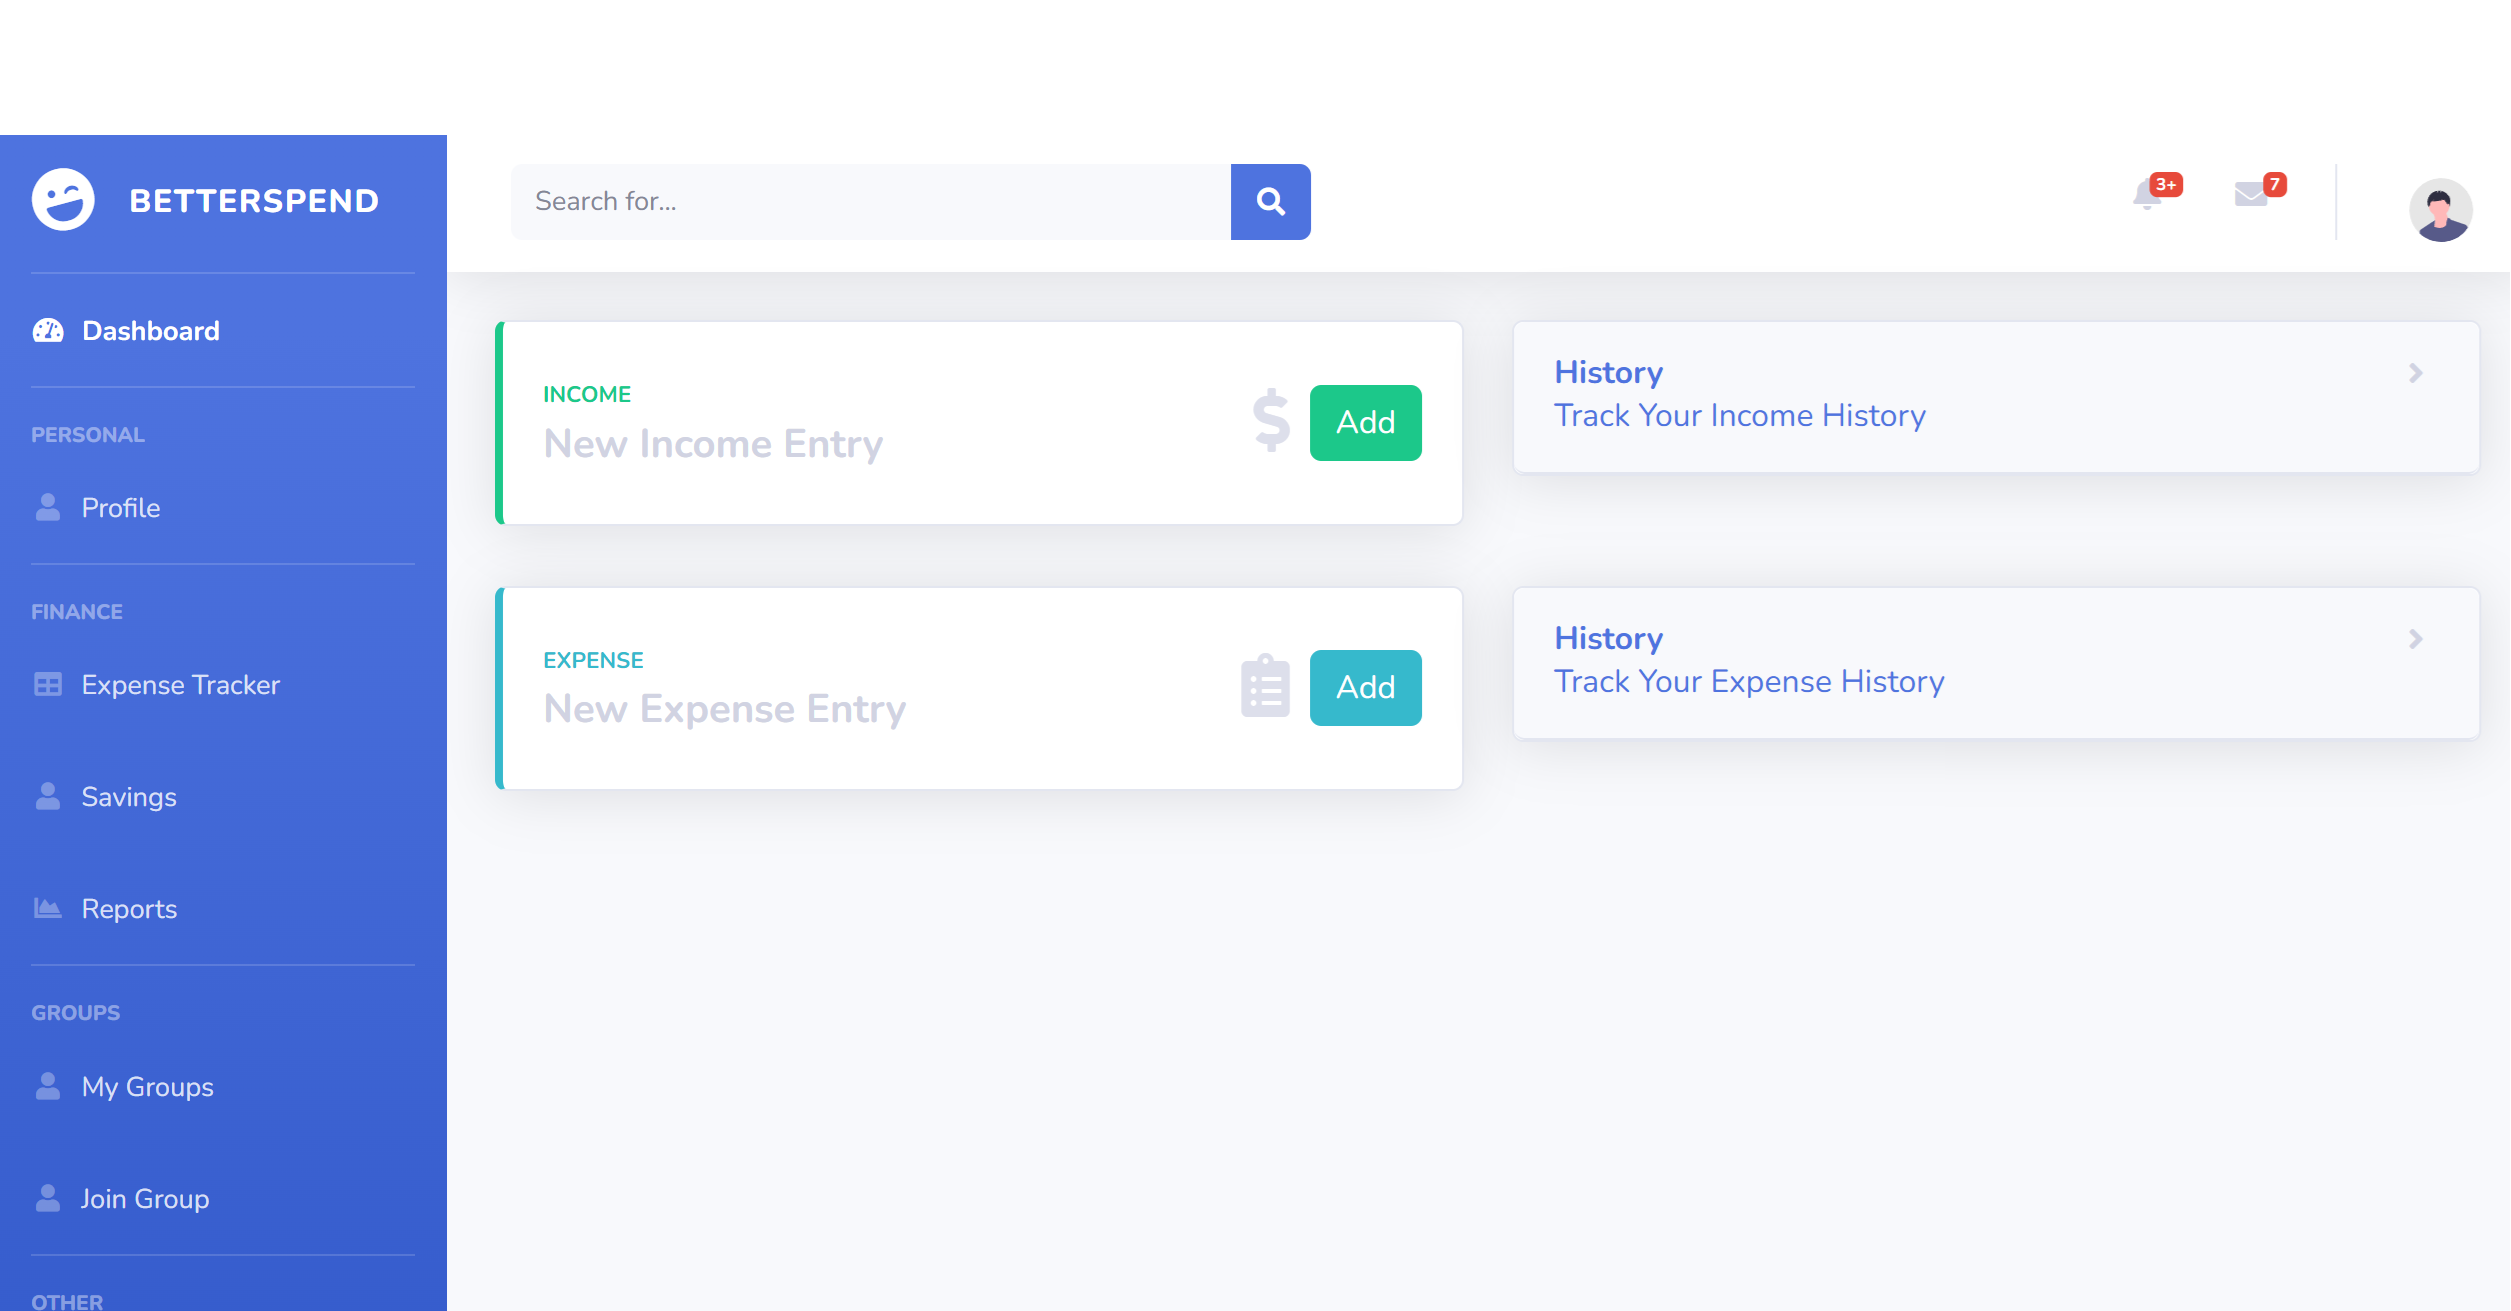
\includegraphics[height=190px]{img/expense-tracker-screenshot}
	\caption{Screenshot: Expense Tracker felület}
	\label{fig:expense-tracker}
\end{figure}

\begin{table}[H]
	\centering
	\begin{tabular}{ | m{0.25\textwidth} | m{0.65\textwidth} | }
		\hline
		\textbf{Funkció} & \textbf{Leírás} \\
		\hline \hline
		\emph{-} & - \\
		\hline
	\end{tabular}
	\caption{Savings oldal}
	\label{tab:savings}
\end{table}

\begin{table}[H]
	\centering
	\begin{tabular}{ | m{0.25\textwidth} | m{0.65\textwidth} | }
		\hline
		\textbf{Funkció} & \textbf{Leírás} \\
		\hline \hline
		\emph{-} & - \\
		\hline
	\end{tabular}
	\caption{Reports oldal}
	\label{tab:reports}
\end{table}

\subsection{Csoportok}
-